\chapter{Evaluation}
In diesem Abschnitt wird darauf eingegangen, unter welchem Szenario der TCP-IP Stack getestet wurde und welche Ergebnisse dabei heraus gekommen sind.
\section{Testaufbau}

Zur Evaluation wurde ein Nexys-Video-FPGA-Entwickler-Board verwendet. Auf diesem wurde Java-Prozessor der AMIDAR-Klasse synthetisiert. Als Netzwerkschnittstelle wurde eine Steckkarte mit zwei Ethernet RJ45 Schnittstellen verwendet. Diese wurde mit einem Patch-Kabel zu der Ethernet Schnittstelle eines Laptops verbunden. Der Laptop verfügt über eine Realtec Gigabit Ethernet Schnittstelle. Des Weiteren läuft auf dem Laptop Ubuntu 16.04 und ein "{}ISC-DHCPD"{} DHCP-Server. Für Testzwecke wurden außerdem diverse Java-Programme genutzt, welche die Java-Netzwerksockel nutzen. 

\subsection{Konfiguration des verwendeten AMIDAR-Systems}
Für die Evaluation wurde ein System mit einer Taktrate von 100MHz verwendet. Dieses entspricht zum dem Zeitpunkt der Abgabe der neusten verfügbaren Konfiguration. Einschließlich des neuen Bus-Systems und Heaps, der über einen deutlich schnelleren Cache verfügt, als die ältere Variante. \\
Ein Nachteil dieser Konfiguration ist, dass ein Scheduler mit reduzierter Funktionalität verwendet wurde, da der alte Scheduler Fehler enthielt, mit denen ein Multithreading fähiger TCP-Stack nicht hätte umgesetzt werden können und der neue Hardware-Scheduler noch nicht einsatzbereit war. Aus diesen Grund könnten sich die hier gemessen Testergebnisse deutlich verbessern, sobald der neue Scheduler eingebaut ist. \\
Des Weiteren wurde zu diesem System über den AMIDAR-Systembuilder ein Ethernet-Controller hinzugefügt, mit dem die angeschlossene Netzwerk-Platine genutzt werden kann.


\begin{figure}
	\centering
	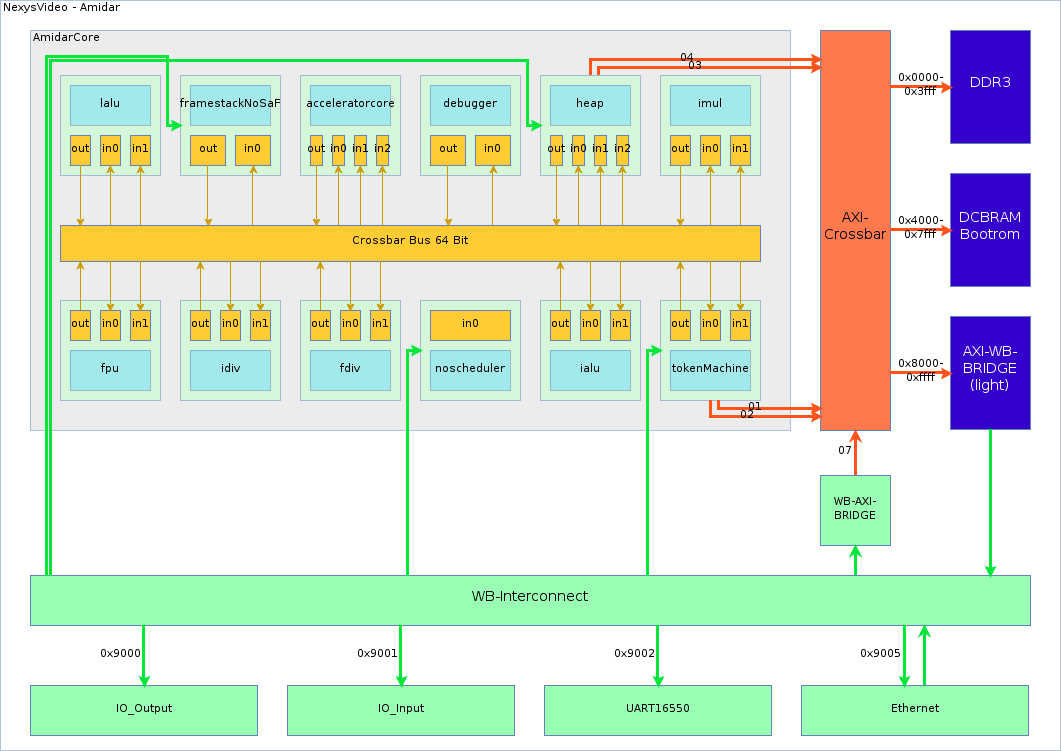
\includegraphics[width = 1\textwidth]{Graphics/system.png}
	\caption{Konfiguration des verwendeten AMIDAR-Systems, automatisch generiert durch den AMIDAR-Systembuilder}

\end{figure}

\FloatBarrier
\section{Grundlegende Funktionen}

Für das Testen der Grundfunktionen wurden mehrere Testszenarien verwendet. Zum einen wurde ein einfacher Echo-Server auf AMIDAR laufen gelassen, der ankommende Wörter zurücksendet. Dieser wurde auf einem oder mehreren Threads aufgeführt. Eine auf dem Laptop laufende Java-Anwendung sendet dabei eingegebene Textnachrichten und wartet auf die Antwort des Servers, welche in der Konsole ausgegeben wird. Dabei wird sowohl der Verbindungsaufbau als auch das Empfangen und Senden von Nachrichten getestet. Dies funktioniert auch mit mehreren offenen Verbindungen parallel. \\\\
Eine Anfrage bei einem DHCP Server funktioniert ebenfalls problemlos, wie sich dem Wireshark Screenshot im Anhang entnehmen lässt. \autoref{DHCP}




\section{Leistung}
Für die Leistungsmessung wird eine Mischung von Daten verwendet, die entweder mit Wireshark ausgelesen wurden, in den Testanwendungen auf dem Laptop in eine .csv Datei geloggt, oder während dem Betrieb auf AMIDAR ermittelt und über UART ausgegeben wurden. 
Die Latenz der einzelnen Pakete wurde Wireshark entnommen. Da Wireshark auf dem Laptop lief, ist die Übertragungszeit des letzten Pakets, das vom Laptop in einem Handshake gesendet wurde nicht gemessen worden. \\
Beim drei Wege Handshake, der von dem Laptop initiiert wurde, betrug die RTT nach dem Senden des SYN-Paketes bis zum Eintreffen des SYN-ACK-Pakets 15-30 Millisekunden. Momentan gibt es eine recht große Schwankung der Reaktionszeit. \\
Falls die Übertragung von AMIDAR initiiert wird, benötigt der Laptop 900 Millisekunden, um auf die Anfrage zu reagieren. Nach weiteren 40 Millisekunden trifft das ACK-Paket von AMIDAR ein.\\\\
In einem weiteren Test wurden zehn Verbindungen zum selben Zeitpunkt geöffnet, über die jeweils in kurzen Abständen 500 Byte an Daten übertragen wurden. Diese Daten wurden von AMIDAR als Echo zurückgesendet. Dieses Szenario soll einen Server-Betrieb simulieren, bei dem Anfragen mehrerer Clients beantwortet werden sollen. Die Latenz dieser Übertragung wurde in einer Logdatei gespeichert und betrug zwischen 1,4 und 3,5 Sekunden. Dabei entfiel der größte Teil der Zeit auf das Auslesen der Daten aus den ankommenden Datenpaketen.\autoref{Multithread}\\

\begin{tabular}{cccc}
\# & Start Time$[ms]$ & End Time $[ms]$ & Response Time$[ms]$\\
1 &1495793145037&	1495793148691&	3654\\
2 &1495793149191&	1495793151370&	2179\\
3 &1495793151871&	1495793153906&	2035\\
4 &1495793154406&	1495793156688&	2282\\
5 &1495793157188&	1495793158886&	1698\\
6 &1495793159387&	1495793160988&	1601\\
7 &1495793161489&	1495793163013&	1524\\
8 &1495793163513&	1495793164989&	1476\\
\end{tabular}\\\\
Auffällig dabei ist, dass die Reaktionszeiten der einzelnen Verbindung mit weiteren Iterationen besser werden. \\
Bei diesem Testszenario wurden mit dem Statistik-Modul der AMIDAR-IDE folgende Werte ermittelt:\\\\
\begin{tabular}{lc}
jumpBytecodes & 16842753\\
total & 545259268 \\
distributedToken & 2004025412 \\
axi.transaction& 1\\
cache.hit & 65793\\
cache.hitrate& 0.996109\\
cache.miss& 257\\
outputFifoEmptyAtferFirstTransaction&16780707
\end{tabular}\\\\
Ein Problem, das bei diesem Versuch sichtbar wurde, ist die schwankende Latenz. Die Dauer eines Timeouts wird bei TCP relativ zur RTT bestimmt. Nach dem schnellen SYN-ACK mit kleinen Paketen wird im PC ein entsprechend kurzes Zeitlimit für Timeouts gesetzt. Das hat zur Folge, dass es zu Neuübertragungen größerer Datenpakete kommen kann, wenn diese auf der Seite des AMIDAR-Prozessors verarbeitet werden müssen, obwohl sie nicht verloren gegangen sind. \autoref{ret} \\\\
Die Übertragungsrate beim Senden wurde ermittelt, in dem ein zufällig generiertes Datenpaket in einer Schleife gesendet wurde. Dabei wird eine Übertragungsrate von 1333 kBit/s erreicht. Die Größe der einzelnen Datenpakete hat dabei nur einen vernachlässigbaren Einfluss auf die Nettoübertragungsrate, was darauf schließen lässt, dass das Bottleneck bei dem Sendepuffer liegt. \\\\
Dabei wurden mit dem Statistik-Modul des Debuggers folgende Werte ermittelt:\\\\
\begin{tabular}{lc}
jumpBytecodes & 537919489\\
total & 545259268 \\
distributedToken & 393412689 \\
axi.transaction& 1\\
cache.hit & 65793\\
cache.hitrate& 0.9960939\\
cache.miss& 258\\
outputFifoEmptyAtferFirstTransaction & 16781085
\end{tabular}






 

 